\documentclass{sigchi}

% Override default copyright strip
\toappear{Permission to make digital or hard copies of all or part of this work for personal or classroom use is granted without fee provided that copies are not made or distributed for profit or commercial advantage and that copies bear this notice and the full citation on the first page. Copyrights for components of this work owned by others than ACM must be honored. Abstracting with credit is permitted. To copy otherwise, or republish, to post on servers or to redistribute to lists, requires prior specific permission and/or a fee.}

% Load basic packages
\usepackage{balance}
\usepackage{graphics}
\usepackage{txfonts}
\usepackage{times}
\usepackage{color}
\usepackage{textcomp}
\usepackage{booktabs}
\usepackage{ccicons}
\usepackage{todonotes}
\usepackage{notoccite}

\usepackage{environ}
\usepackage{amsmath}
\usepackage{amssymb}
\usepackage{mathtools}
\usepackage{xcolor}
\usepackage{tikz}
\usetikzlibrary{calc}
\usetikzlibrary{shapes.geometric}

\PassOptionsToPackage{hyphens}{url}
\usepackage[pdftex]{hyperref}

% Define a global style for URLs, rather that the default one
\makeatletter
\def\url@leostyle{%
  \@ifundefined{selectfont}{\def\UrlFont{\sf}}{\def\UrlFont{\small\bf\ttfamily}}}
\makeatother
\urlstyle{leo}

% To make various LaTeX processors do the right thing with page size
\def\pprw{8.5in}
\def\pprh{11in}
\special{papersize=\pprw,\pprh}
\setlength{\paperwidth}{\pprw}
\setlength{\paperheight}{\pprh}
\setlength{\pdfpagewidth}{\pprw}
\setlength{\pdfpageheight}{\pprh}

% Make sure hyperref comes last of your loaded packages, to give it a
% fighting chance of not being over-written, since its job is to
% redefine many LaTeX commands.
\definecolor{linkColor}{RGB}{6,125,233}
\hypersetup{%
    pdftitle={SIGCHI Conference Proceedings Format},
    pdfauthor={LaTeX},
    pdfkeywords={SIGCHI, proceedings, archival format},
    bookmarksnumbered,
    pdfstartview={FitH},
    colorlinks,
    citecolor=black,
    filecolor=black,
    linkcolor=black,
    urlcolor=linkColor,
    breaklinks=true,
}

% For scaling down tikzpictures
\makeatletter
\newsavebox{\measure@tikzpicture}
\NewEnviron{scaletikzpicturetowidth}[1]{%
  \def\tikz@width{#1}%
  \def\tikzscale{1}\begin{lrbox}{\measure@tikzpicture}%
  \BODY
  \end{lrbox}%
  \pgfmathparse{#1/\wd\measure@tikzpicture}%
  \edef\tikzscale{\pgfmathresult}%
  \BODY
}
\makeatother

% Size of the component blocks
\newlength{\blockSize}
\setlength{\blockSize}{1.5cm}

% Style of block component in diagram
\tikzset{Component/.style={minimum width=\blockSize,
                           minimum height=\blockSize,
                           text width=\blockSize,
                           align=center}}

% Style of flow arrow in diagram
\tikzset{Flow Arrow/.style={blue, dotted, line width=1pt}}

\begin{document}

\title{AtmoSPHERE}

\numberofauthors{1}
\author{%
    \alignauthor{Jay Feng, William Hwang, Joseph Wu, Mingyu Zhang \\
        \affaddr{CSE 477, Spring 2015}} \\
}

\maketitle

\begin{abstract}
    Air quality is an upstream component of human health, which cannot be addressed through primary care health facilities.
    In this work, we present AtmoSPHERE, a connected, wearable air monitor.
    Our system is comprised of a wrist-worn sensor suite, a connected smartphone, and a cloud service.
    The sensor suite measures two major categories of airborne health risks: particulate matter and volatile organics.
    The phone tags the data with location data and is used to communicate between the sensors and cloud.
    From the cloud service, we display a dashboard to highlight air quality in travelled areas.
    To evaluate the system, we collected data from 2 users over the course of a week of normal activity.
\end{abstract}

\category{J.3}{Health}{}

\keywords{Air quality; Upstream health; Wearable; Connected devices; Distributed sensors.}

\section{Introduction}
% Background/Motivation
Approximately half of all known health conditions originate from environmental factors\cite{Manchanda:TEDTalk}.
These factors are generally labelled ``upstream'' factors due to how they are detached from a person's immediate symptoms during illness.
Upstream factors include variables such as the sanitation of a person's home, the condition of their workplace, or the local air.
The existing health care system is not equipped to handle issues outside the hospital or clinic.
However, many upstream factors are simple to identify, straight forward to address.
We envision a device that can inform the user and others in the vicinity about one subset of upstream health risks.

% PM sensor background
In this project, we introduce AtmoSPHERE, a wearable air monitor for both particulate matter and volatile organic compounds (VOC).
Particulate matter (PM), is any microscopic matter suspended in the atmosphere.
Particulates include dust as well as more dangerous varieties classified by their diameter in microns, known as PM10 and PM2.5.
A PM sensor is comprised of an infrared emitting diode and a phototransistor placed diagonally\cite{PMSensor:Datasheet}.
As particles pass through the path between the two components, deflected light is recorded by the phototransistor.
This approach can detect visible dust as well as finer particles, such as PM2.5.

% VOC sensor background
Volatile organic compounds (VOC) are compounds with high vapor pressure at room temperature.
VOCs are numerous and varied, and include harmful compounds such as benzene, chlorofluorocarbons, and methylene chloride.
A VOC sensor comes in many forms.
A semiconductor VOC sensor uses a chemical reaction between the air and a heated substrate, such as Tin Dioxide\cite{VOCSensor:Datasheet}.
As the concentration of VOC in the air increases, the corresponding resistance of the substrate drops by a measurable amount.

% Advantages of a wearable
AtmoSPHERE is intended to allow distributed sensing of environmental risks.
The wearable is linked to a smartphone and through that, our cloud service and data API.
By aggregating data from multiple users, we can build substantial maps of local air quality.
We expect this device can be used to inform lifestyle changes.

\section{Theory of Operation}
% How to wear it
The only physical requirement of the AtmoSPHERE is sufficient air flow through the device.
The wearable is designed to be worn on the wrist, where the movement of the arms will agitate air into the sensors.
However, the device can be attached to any other location on the body.
The wearable also doubles as a stationary air monitor, such as when taken off during charging.
While stationary, diffusion is also an acceptable means of passing air over the sensor.

% Phone companion
For data collection, the wearable should always be within a short distance of a paired Android phone.
The wearable and phone communicate via Bluetooth, so the maximum separation of the two devices should not exceed 10 meters.
At the same time, the phone should have location services enabled and at least an intermittent internet connection.

\section{Implementation Details}
In this section, we will detail the hardware design, the software features, and the data API.
Figure~\ref{fig:software block} shows the overall system architecture and data flow.
\begin{figure}
    \centering
    \begin{scaletikzpicturetowidth}{0.9\columnwidth}
\begin{tikzpicture}[scale=\tikzscale, every node/.style={scale=\tikzscale}]
    % Most of the specialized hardware
    \node[draw, rectangle, Component]
        at (0, 0) (Embedded) {Wearable \\ Device};

    % Phone for GPS and data connection
    \node[draw, rectangle, Component, anchor=west]
        at ($(Embedded.east) + (2, 0)$) (Phone) {Phone};

    % Web server
    \node[draw, rectangle, Component, anchor=north]
        at ($(Phone.south) - (0, 1)$) (Server) {Web \\ Server};

    % Database
    \node[draw, cylinder, shape border rotate=90, aspect=0.25, Component, anchor=east]
        at ($(Server.west) - (2, 0)$) (Database) {Database};

    % Client
    \node[draw, rectangle, Component, anchor=west]
        at ($(Server.east) + (1, 0)$) (Client) {Client \\ Computer};

    % Primary interconnect between hardware & software systems
    \draw[->, Flow Arrow] (Embedded) -- (Phone)
        node[black, pos=0.5, sloped, above] {Bluetooth};

    % Data flow
    \draw[->, Flow Arrow] (Phone) -- (Server)
        node[black, pos=0.5, left] {Sensor Data + GPS};
    \draw[-, Flow Arrow, opacity=0.3] (Server.north) to[out=south, in=east] (Server.west);
    \draw[<->, Flow Arrow] (Server) -- (Database);
    \draw[-, Flow Arrow, opacity=0.3] (Server.south) to[out=north, in=east] (Server.west);
    \draw[->, Flow Arrow] (Server) -- (Client);

\end{tikzpicture}
\end{scaletikzpicturetowidth}

    \caption{System architecture and data flow.}
    ~\label{fig:software block}
\end{figure}

\subsection{Hardware}
% Description of hardware
The device captures a total of four variables: PM, VOC, temperature, and humidity.
The PM sensor is the Sharp GP2Y1010AU0F.
The VOC sensor is the AMS AS-MLV-P2.
Temperature and humidity are captured together with the Amphenol ChipCap2.
We used a TinyDuino Processor Board to collect the sensor values and a TinyShield Bluegiga BLE112 Bluetooth module to communicate with the phone (Figure~\ref{fig:hardware block}).
A RGB LED is used to alert the user in case any sensor values peak.

% Description of power
For the power source, we used a Lithium Ion Polymer battery.
Due to the different voltage requirements of the sensors and microprocessor, the battery is attached to a boost converter, NCP1402, for most of the components; and a buck converter, ISL85415, for the VOC sensor.
For charging the device, we added a Basic Micro-USB LiPo Charger.
A switch toggles the connection to the battery, although the device is expected to stay powered continuously.
All of the components are placed in a 3D-printed case (see Figure~\ref{fig:housing}).
The fully assembled wearable is shown in Figure~\ref{fig:device open}.
\begin{figure}
    \centering
    \begin{scaletikzpicturetowidth}{0.9\columnwidth}
\begin{tikzpicture}[scale=\tikzscale, every node/.style={scale=\tikzscale}]
    % Sensor hub
    \node[draw, rectangle, Component]
        at (0, 0) (Arduino) {Arduino};

    % Output module
    \node[draw, rectangle, Component, anchor=west]
        at ($(Arduino.east) + (1, 0)$) (Bluetooth) {Bluetooth};

    % Sensors
    \node[draw, rectangle, Component, anchor=north]
        at ($(Bluetooth.south) - (0, 1)$) (PM Sensor) {PM \\ Sensor};
    \node[draw, rectangle, Component, anchor=south]
        at ($(Bluetooth.north) + (0, 1)$) (Humidity) {Humidity \\ Sensor};
    \node[draw, rectangle, Component, anchor=south]
        at ($(Arduino.north) + (0, 1)$) (Gas Sensor) {Gas \\ Sensor};

    % Power
    \node[draw, rectangle, Component, anchor=east]
        at ($(Arduino.west) - (1, 0)$) (Booster) {Boost \\ Converter};
    \node[draw, rectangle, Component, anchor=east]
        at ($(Gas Sensor.west) - (1, 0)$) (Bucker) {Buck \\ Converter};
    \node[draw, rectangle, Component, anchor=east]
        at ($($(Booster.west)!0.5!(Bucker.west)$) - (1, 0)$) (Power) {Battery};
    \node[draw, rectangle, Component, anchor=north]
        at ($(Power.south) - (0, 1)$) (Charger) {Micro-USB \\ Charger};

    % Sensor interconnects
    \draw[->, Flow Arrow] (PM Sensor) -- (Arduino)
        node[pos=0.5, right] {Digital};
    \draw[->, Flow Arrow] (Humidity) -- (Arduino)
        node[pos=0.5, right] {I$^2$C};
    \draw[->, Flow Arrow] (Gas Sensor) -- (Arduino)
        node[pos=0.5, left] {Analog};

    % Power lines
    \draw[->, Flow Arrow] (Charger) -- (Power);
    \draw[->, Flow Arrow] (Power) -- (Booster) -- (Arduino);
    \draw[->, Flow Arrow] (Power) -- (Bucker) -- (Gas Sensor);

    % To phone
    \draw[->, Flow Arrow] (Arduino) -- (Bluetooth);

\end{tikzpicture}
\end{scaletikzpicturetowidth}

    \caption{Components of the wearable device.}
    ~\label{fig:hardware block}
\end{figure}
\begin{figure}
    \centering
    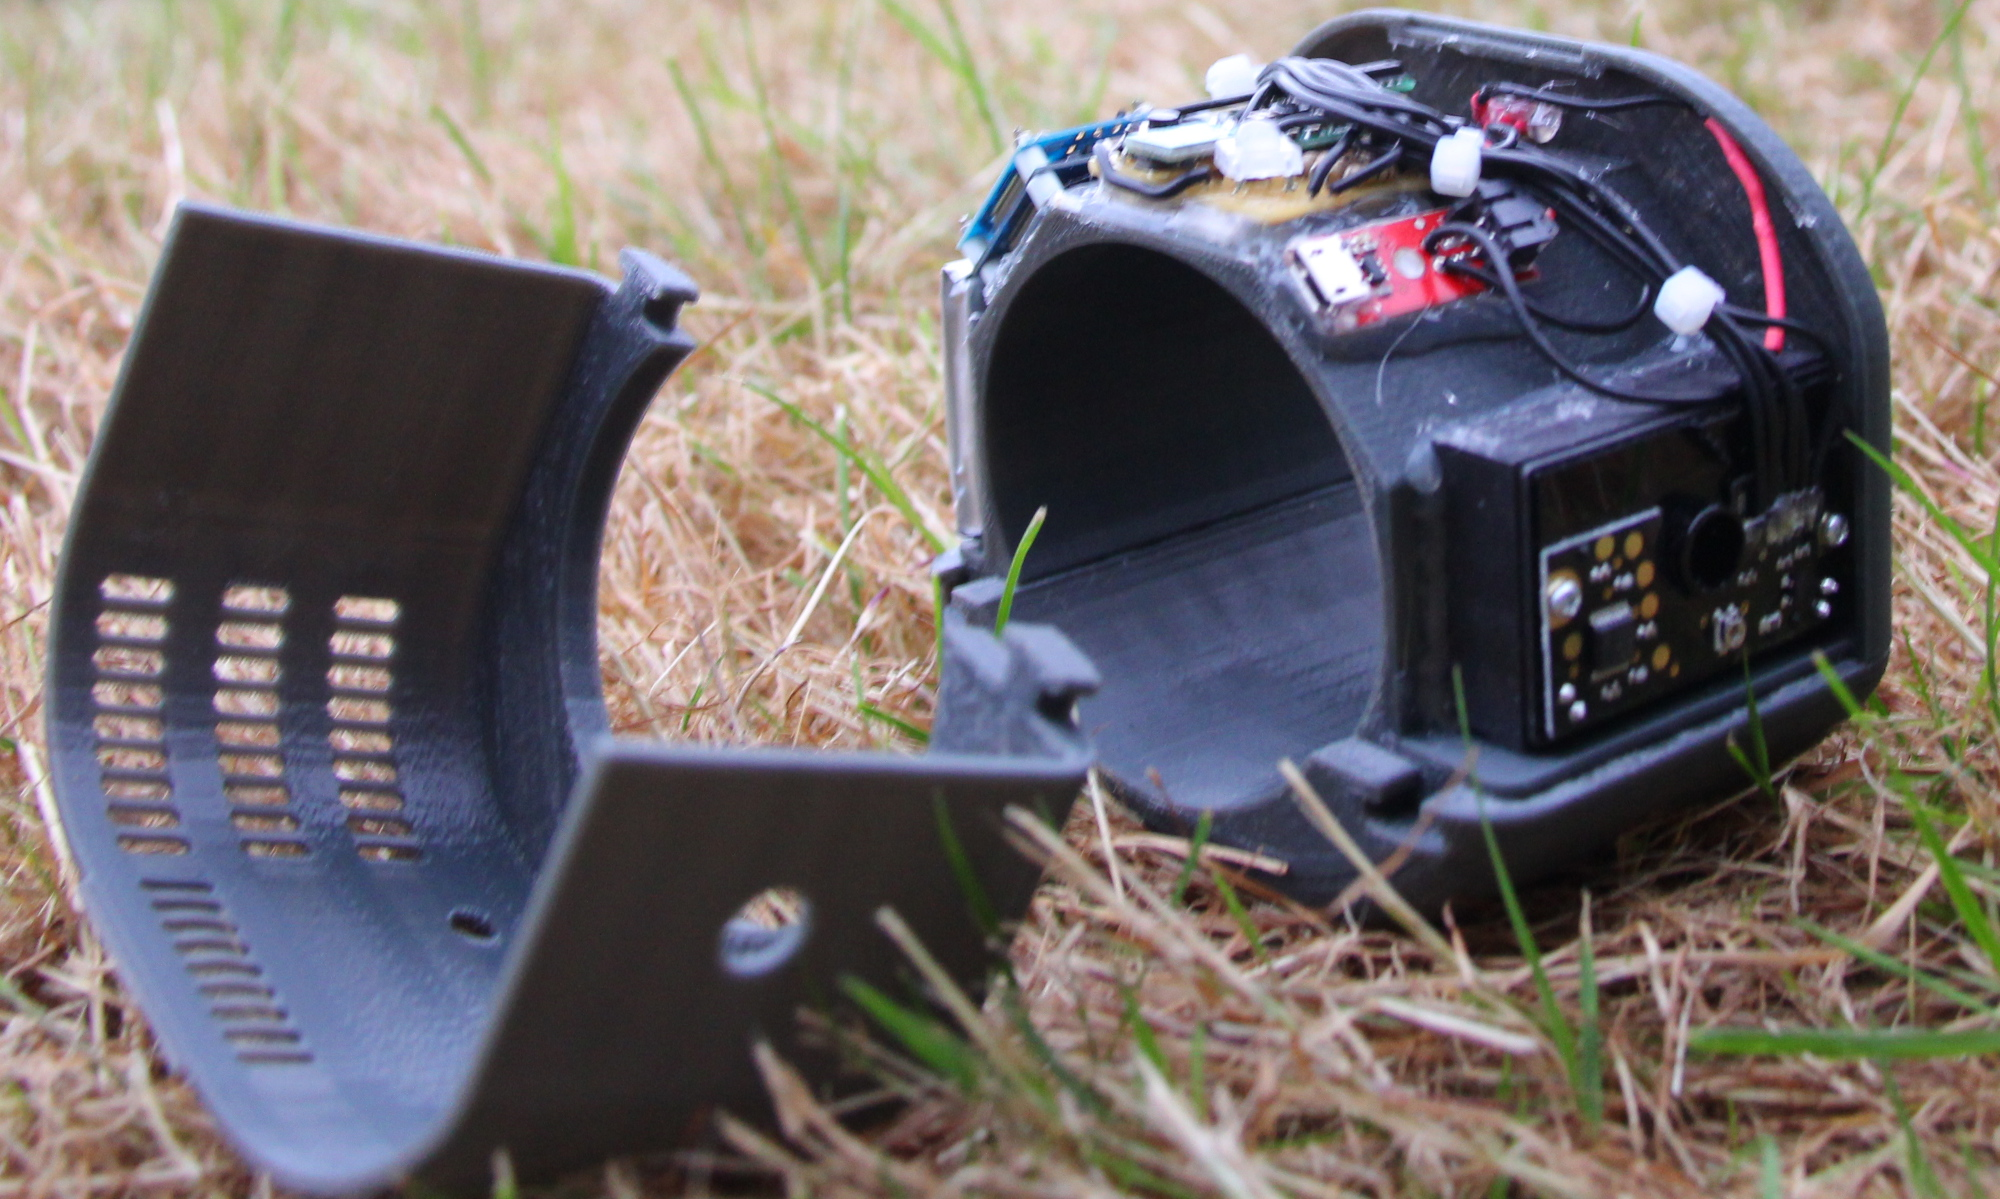
\includegraphics[width=0.9\columnwidth]{figures/Device-Open.jpg}
    \caption{Fully assembled prototype AtmoSPHERE with an open case.
        Starting from the right, we see the PM sensor, Micro-USB charger, proto-board, Arduino, and battery.}
    ~\label{fig:device open}
\end{figure}

\subsection{Phone Application}
To connect our device with the cloud services, we require an Android phone of at least version 4.3.1 (Jelly Bean).
This version of Android has built-in support for Bluetooth Low Energy, which we is used to communicate between the phone and wearable.
The Android application consists of four screens:
\begin{itemize}
    \item The welcome screen performs some preliminary checks on the services the app requires, such as an internet connection and location services.
    \item The login screen authenticates the user grants the phone access to our cloud services.
    \item The Bluetooth screen scans and connects to our device.
    \item The data display screen shows several views of the data from the sensor.
        The display is fairly simple; more substantial views are available on our associated web site.
\end{itemize}
The Bluetooth connection is managed with a foreground service.
This service reads data from the wearable and pushes the data onto the cloud.
When an internet connection is not available, the data is stored locally until an internet connection becomes available.

\subsection{Web Application}
The web interface is built with Django.
A simple user registration and login interface exists for differentiating between each user's datapoints.
The primary web interface is a dashboard of three data displays: a heat map, timeline, and histogram.
Data is shown over the last day or week, or all existing data is shown.
Only one attribute collected by the wearable, i.e. PM or VOC, is displayed at once.
\begin{figure}
    \centering
    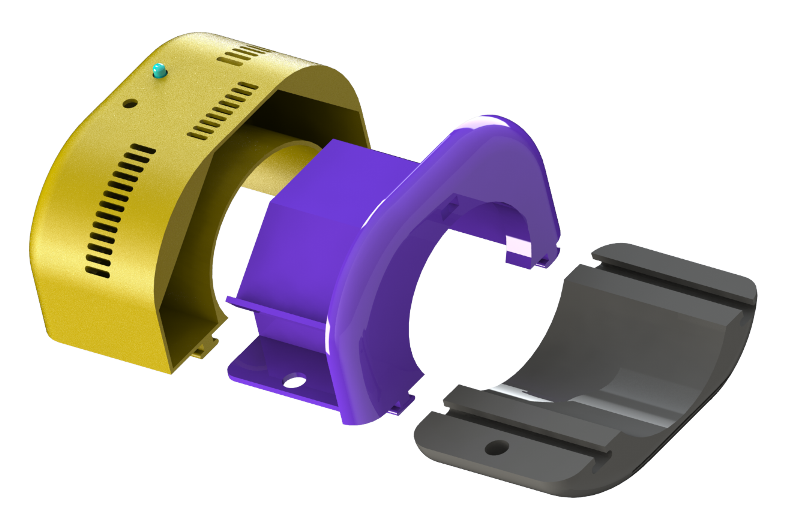
\includegraphics[width=0.9\columnwidth]{figures/Mechanical-Housing.png}
    \caption{CAD rendering of the housing for AtmoSPHERE.}
    ~\label{fig:housing}
\end{figure}

\subsection{Data API}
The cloud services follow a REST pattern and are linked to the web interface through a different endpoint.
\begin{itemize}
    \item \verb|GET /data/| -- Returns a list of datapoints gathered by the sensors
    \item \verb|GET /data/user/| -- Returns a list of datapoints gathered by the current user
    \item \verb|POST /data/| -- Adds a single datapoint to the database
\end{itemize}
The two \verb|GET| endpoints can be further filtered with a query string:
\begin{itemize}
    \item xmin -- Number.  Minimum longitude of the data.
    \item xmax -- Number.  Maximum longitude of the data.
    \item ymin -- Number.  Minimum latitude of the data.
    \item ymax -- Number.  Maximum latitude of the data.
    \item before -- Date (Format: YYYY-MM-DD HH:MM:SS).  Maximum timestamp of the data.
    \item after -- Date (Same format as above).  Minimum timestamp of the data.
    \item o -- ``timestamp''.  If present, sorts the results in ascending order by time.
\end{itemize}

\section{Results}
We built two prototype devices and gathered data over a week in the vicinity of the University of Washington and Seattle.
We expected and observed low levels for PM.
We also expected low levels for VOC, however observed values showed high levels of VOC around some roads and within some buildings (see Figure~\ref{fig:voc heatmap}).
In addition, we had several users wear the device during their daily activity.
One such example is shown in Figure~\ref{fig:commute}.
\begin{figure}
    \centering
    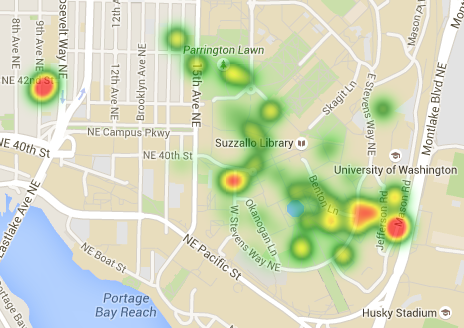
\includegraphics[width=0.9\columnwidth]{figures/VOC-Heatmap.png}
    \caption{VOC data represented as a heatmap.
        Red represents high levels, yellow intermediate, green low.}
    ~\label{fig:voc heatmap}
\end{figure}
\begin{figure}
    \centering
    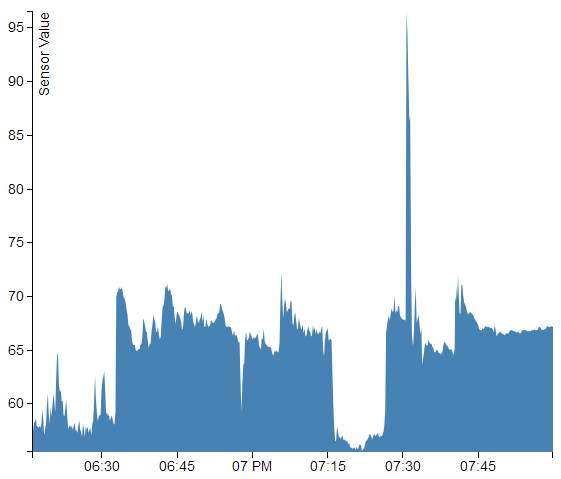
\includegraphics[width=0.9\columnwidth]{figures/Commute-Timeline.png}
    \caption{VOC levels over a long commute from the University of Washington to the subject's home.
        Levels appear lower when outside walking.
        Elevated levels appear when inside a bus and in the subject's house.
        The spike is due to the subject washing his hands with (perfumed) hand soap.}
    ~\label{fig:commute}
\end{figure}

\section{Challenges}
In terms of hardware challenges, minimizing the form factor of the device posed the greatest challenge.
The PM sensor in particular requires a set amount of space in order to function properly, due to the optical requirements of the sensor.
Smaller versions of PM sensors are physically possible\cite{PMSensor:Article}, but such sensors are not commercially available as of yet.
Instead, we determined that the form factor was less important than a working prototype.
As a result, the overall size of the prototype device was increased (see Figure~\ref{fig:housing}).

The VOC sensor exhibited some drift over time.
With two devices, we could cross reference the sensor values against each other.
PM, temperature, and humidity values all agreed within 2\% of one other if the two devices are adjacent.
However, the VOC sensor could be significantly divergent.

\section{Future Work and Discussion}
The future of the air quality monitoring system will mostly face challenges with adoption and widespread use.
While having a local air quality monitor tracking activity at all times is potentially beneficial for personal health monitoring, the amount of accuracy increases as more and more users track air quality in the same region.
With more users, gaps in coverage are overcome.
At the same time, anomalies, such as from people blowing in the device or leaving it unattended by a pollution source, can be averaged away.
After all, the variability and noise is large on any single device.

If the device is slimmed down to make it more wearable and friendly to use (see Figure~\ref{fig:device worn} for the current prototype), it can serve to prevent unhealthy behavior on a macro scale, or just increase awareness of unhealthy areas.
With lots of crowd-sourced data, users can be alerted for a variety of environmental concerns that interfere with their daily lives.
These alerts would probably be for risks that lower health outcomes over the long term.
For example, a high particle count may indicate high pollen areas to avoid, or some large scale construction work in the area.
\begin{figure}
    \centering
    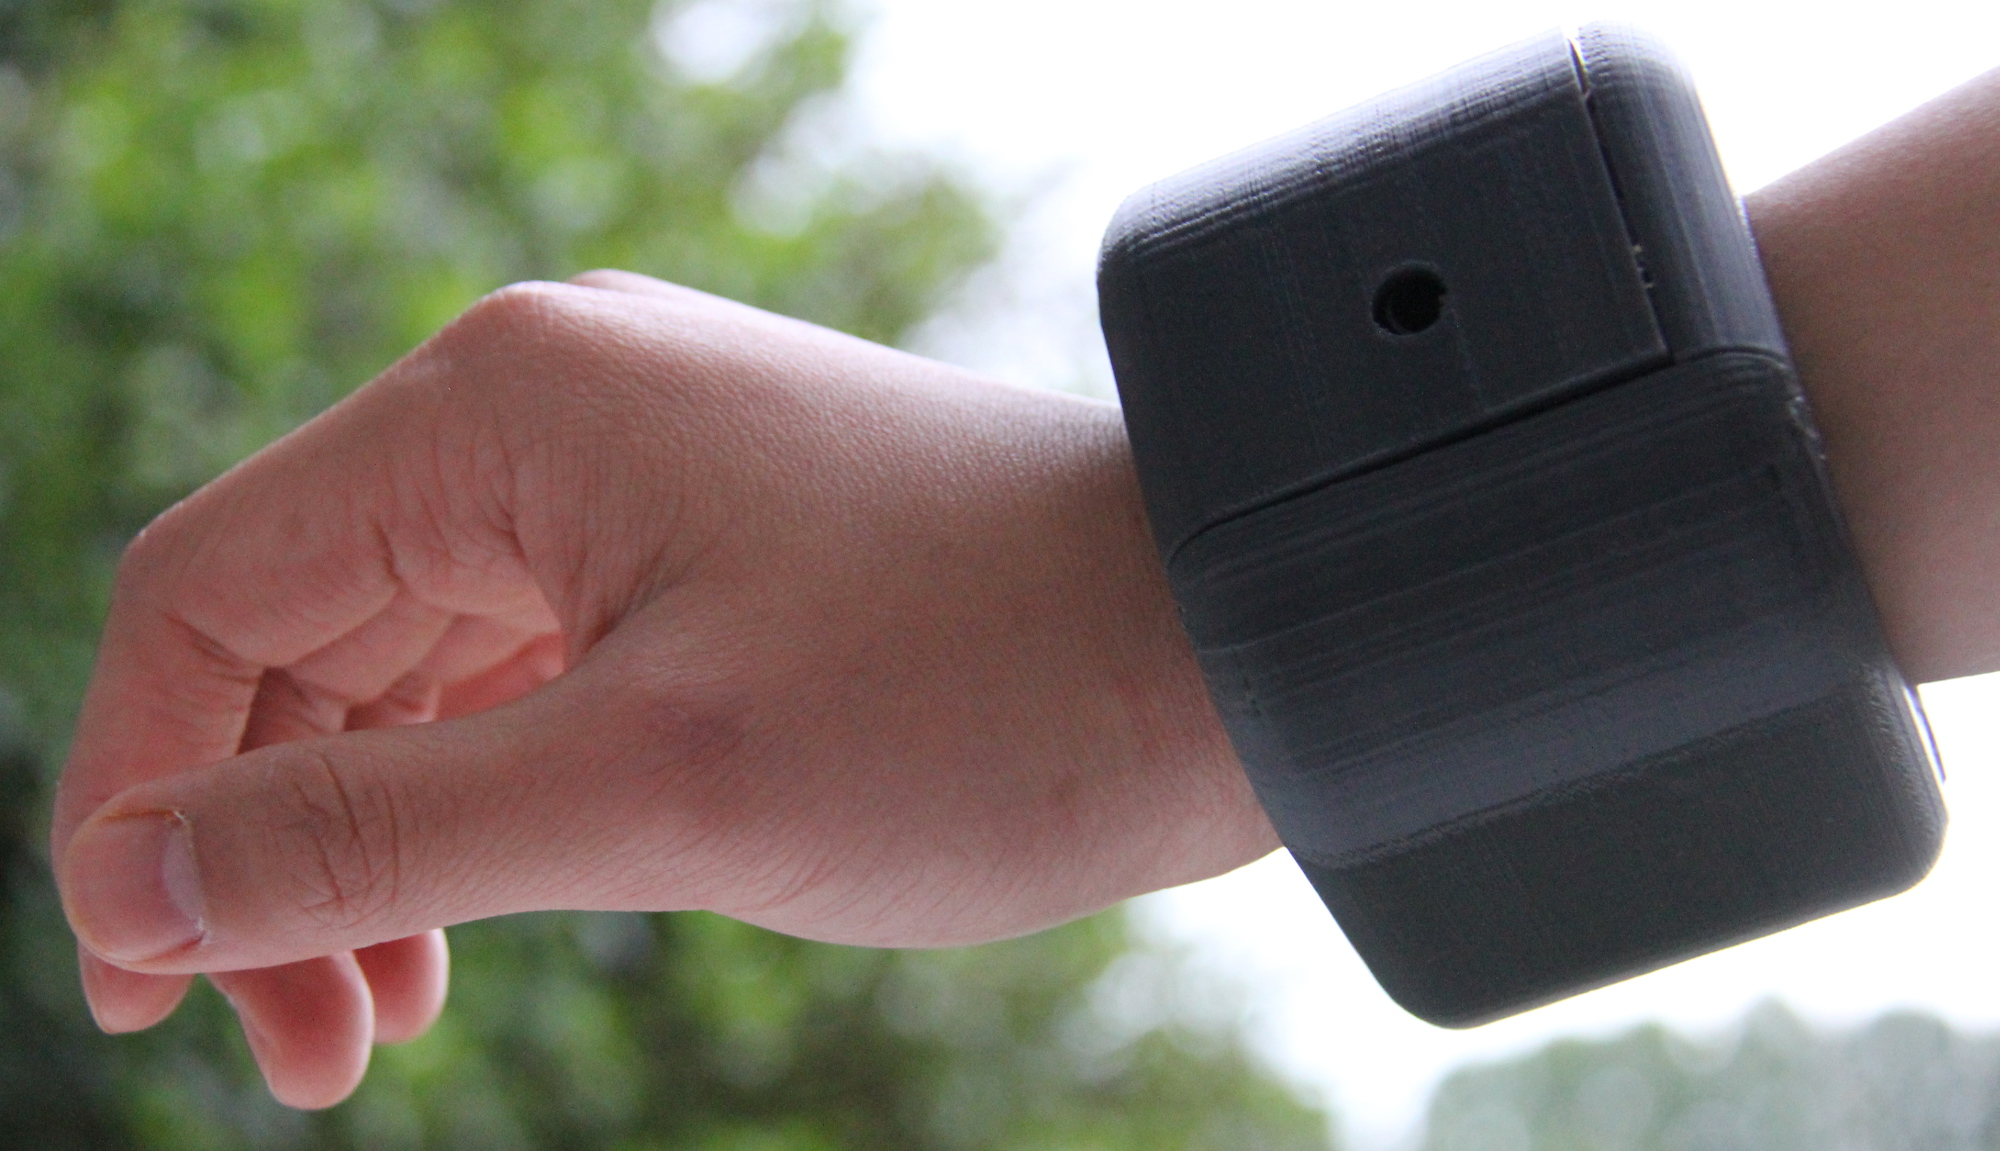
\includegraphics[width=0.9\columnwidth]{figures/Device-Worn.jpg}
    \caption{Fully assembled prototype AtmoSPHERE, worn on the wrist.}
    ~\label{fig:device worn}
\end{figure}

A significant market for air quality monitors exists in the developing world.
Seattle is relatively clean and free of egregious pollution (see Figure~\ref{fig:mueller}).
The city hosts ``green'' initiatives often, and has high air quality standards for a city of its size.
On the other hand, approximately 3.5 million deaths each year are attributed to air pollution in India alone\cite{AirPollution:Article}.
For countries in this situation, an increased number of monitors gives grass-root support for environmental initiatives.
\begin{figure}
    \centering
    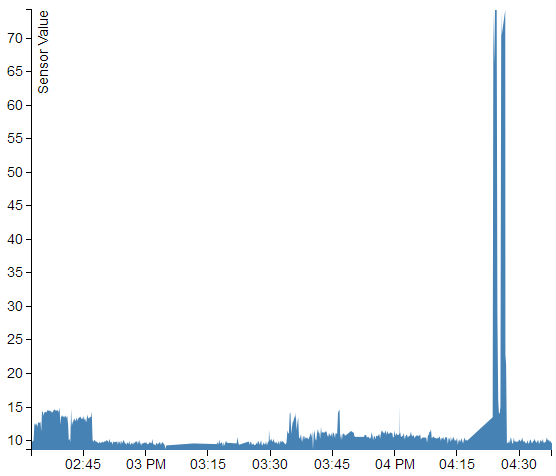
\includegraphics[width=0.9\columnwidth]{figures/Mueller-Timeline.png}
    \caption{In Seattle, it is very difficult to get a high PM reading.
        To get the spikes in the timeline above, the subject entered a workshop in Mueller hall in the University of Washington, while someone was performing experiments with flaky materials.}
    ~\label{fig:mueller}
\end{figure}

The necessity of air monitoring devices is clear; the true challenge is making the device practical and accessible for low-income and poverished countries where the people need it the most.
The bill of materials for an air quality monitor is quite significant.
Our device cost \$165 for parts alone.
Even if made at scale, the price is unlikely to drop below \$100.
This is evidenced by the price point of various other air quality monitors available on the market, such as Speck\cite{Competitor:Speck} or TZOA\cite{Competitor:TZOA}.
Considering that a companion smartphone is a usual requirement of such devices, such air quality monitors are currently far from marketing to developing countries.

\section{Conclusion}
The AtmoSPHERE device allows a user to track and monitor the air pollution in their life using four different environmental sensors.
With the wide array of sensor types, the device has a lot of potential to showcase environmental standards across cities and crowd-source data that would otherwise be hard to connect.
Air pollution will increasingly become a concern in countries such as China and India.
In the U.S. topics such as climate change will also call for increased awareness over the environment.
And ubiquitous air monitoring systems should become more of a commonality.

% Try to balance the columns of the last page
\balance{}

\bibliographystyle{SIGCHI-Reference-Format}
\bibliography{report}

\end{document}
